% NeurIPS 2026 Evaluations & Datasets Track Submission
\documentclass{article}
\usepackage[eandd]{neurips_2026}

\usepackage{graphicx}
\usepackage{booktabs}
\usepackage{multirow}
\usepackage{amsmath}
\usepackage{url}
\usepackage{hyperref}
\usepackage{xcolor}

\title{From BM25 to Corrective RAG: Evaluating Retrieval Strategies for Heterogeneous Text-and-Table Documents}

\author{
  Meftun Akarsu \\
  Technische Hochschule Ingolstadt \\
  \texttt{mea5963@thi.de} \\
  \And
  Recep Kaan Karaman \\
  Uludag University \\
  \texttt{kaankaraman@uludag.edu.tr} \\
  \And
  Christopher Mierbach \\
  Radiate \\
  \texttt{christopher@radiate.com}
}

\begin{document}
\maketitle

\begin{abstract}
A RAG pipeline is only as good as the documents it retrieves, yet retrieval on corpora that mix prose and tables has received little empirical study. MTEB and BEIR evaluate on homogeneous text, where dense retrieval generally wins; it is unclear how much of that ordering survives on documents whose answers live in table cells. We evaluate nine retrieval methods on T\textsuperscript{2}-RAGBench, a financial QA benchmark of 23,088 queries over 7,318 SEC-filing documents, plus an open-weight BGE-M3 stack as a robustness check on encoder choice, and report Recall@$k$, MRR, nDCG, end-to-end Number Match, and paired bootstrap significance tests.

Four results stand out. BM25 beats \texttt{text-embedding-3-large} on nearly every metric, inverting the MTEB/BEIR ordering. Hybrid RRF followed by a cross-encoder reranker reaches Recall@5 = 0.816 and MRR@3 = 0.605, well ahead of any single-stage method. HyDE and multi-query expansion hurt rather than help: hallucinated numbers pull the query embedding away from documents with the exact figure. And of the 31\% of queries whose gold document is missed at rank 5, 73\% fail for the same reason---the answer is a table cell that the encoder cannot recover from linearized text. We release the evaluation code, prompts, FAISS indices, and per-query outputs.
\end{abstract}

% ============================================================
\section{Introduction}
\label{sec:intro}

In a RAG system \citep{lewis2020rag}, a retriever supplies the context an LLM conditions on. If the retriever misses the relevant document, no amount of prompt engineering recovers the answer: retrieval sets a hard upper bound on the whole pipeline. Most RAG research nevertheless treats retrieval as a solved substrate and focuses attention on prompting, decoding, and judging.

\paragraph{The gap for text-and-table corpora.}
That assumption breaks down on documents that mix prose and tables. Financial filings, earnings reports, and regulatory documents are built this way: the prose carries context, the tables carry the numbers. Answering \emph{``What was the 2019 year-over-year revenue growth?''} requires finding both the right document and the right cell inside it. The benchmarks most practitioners consult---MTEB \citep{muennighoff2023mteb} and BEIR \citep{thakur2021beir}---evaluate on homogeneous text, where dense retrieval usually outperforms sparse baselines. Whether that ordering survives a shift to heterogeneous documents is an open empirical question, and our main finding is that it does not.

We use T\textsuperscript{2}-RAGBench \citep{strich2026t2ragbench}, a financial QA benchmark of 23{,}088 queries over 7{,}318 documents. The original paper evaluated six retrieval methods with two metrics; we evaluate nine methods plus an open-weight BGE-M3 robustness panel, and report the full retrieval and generation metric suite along with paired bootstrap significance tests.

\paragraph{Contributions.}
\begin{enumerate}
    \item A head-to-head evaluation of nine retrieval methods on T\textsuperscript{2}-RAGBench, covering sparse, dense, hybrid, cross-encoder-reranked, query-side, index-side, and adaptive pipelines, with paired bootstrap significance tests, plus an open-weight BGE-M3 stack as a robustness check on encoder choice.
    \item Evidence that rankings on MTEB and BEIR do not transfer to text-and-table data: BM25 beats a strong dense encoder (\texttt{text-embedding-3-large}) on nearly every metric.
    \item An error analysis of 100 sampled retrieval failures showing that 73\% stem from a single cause---the answer is a table cell that serialized-text encoders cannot locate---which we argue is the next concrete open problem in this area.
    \item Two negative results: HyDE and multi-query expansion degrade retrieval on numerical financial queries, and CRAG-style correction does not close the gap to hybrid fusion.
    \item Ablations on fusion type and reranker candidate depth, plus a released evaluation framework with prompts, indices, and per-query outputs.
\end{enumerate}

% ============================================================
\section{Related Work}
\label{sec:related}

\paragraph{RAG retrieval methods.}
BM25 remains competitive in zero-shot settings \citep{thakur2021beir}. Dense dual-encoders \citep{karpukhin2020dpr} and their successors---E5 \citep{wang2022e5}, E5-Mistral \citep{wang2024e5mistral}, BGE-M3 \citep{chen2024bgem3}---advance MTEB rankings through contrastive pretraining. Hybrid retrieval fuses sparse and dense signals via RRF \citep{cormack2009rrf}, consistently improving recall by 15--30\% \citep{li2025ragbestpractices}. Two-stage reranking with cross-encoders further refines results \citep{gao2024ragsurvey}. Query-side methods include HyDE \citep{gao2022hyde} and RAG-Fusion \citep{raudaschl2023ragfusion}. Index-side methods include Contextual Retrieval \citep{anthropic2024contextual} and HyPE \citep{vake2025hype}. Adaptive approaches like CRAG \citep{yan2024crag} trigger corrective searches when confidence is low.

\paragraph{Text-and-table QA.}
HybridQA \citep{chen2020hybridqa} introduced multi-hop reasoning over linked tables and passages. In the financial domain, FinQA \citep{chen2021finqa}, TAT-QA \citep{zhu2021tatqa}, and ConvFinQA \citep{chen2022convfinqa} target numerical reasoning over hybrid contexts. A recent survey \citep{nan2025tableqasurvey} finds that retrieval of heterogeneous context remains the primary bottleneck.

\paragraph{RAG benchmarks.}
BEIR \citep{thakur2021beir} established zero-shot retrieval evaluation across 18 datasets. Recent RAG benchmarks include RGB \citep{chen2024rgb}, CRAG \citep{yang2024crag}, and RAGBench \citep{friel2024ragbench}. \citet{li2025ragbestpractices} study RAG design choices at COLING 2025. None focus on retrieval method comparison over documents with mixed text-and-table content. T\textsuperscript{2}-RAGBench \citep{strich2026t2ragbench} unifies FinQA, ConvFinQA, and TAT-DQA into 23,088 queries over 7,318 financial documents; where the original paper tested six methods with two metrics, we evaluate nine methods plus an open-weight BGE-M3 robustness panel, with a comprehensive set of retrieval and generation metrics.

% ============================================================
\section{Methodology}
\label{sec:method}

\subsection{Dataset}
\label{sec:dataset}

T\textsuperscript{2}-RAGBench \citep{strich2026t2ragbench} contains 23,088 question-context-answer triples from FinQA (8,281), ConvFinQA (3,458), and TAT-DQA (11,349), covering 7,318 unique financial documents averaging $\sim$920 tokens each. Each document mixes text and markdown-formatted tables from SEC filings. The benchmark reformulated all questions using Llama 3.3-70B to incorporate identifying information (company name, sector, report year), producing questions with exactly one correct answer regardless of context. All answers are numerical. The original best method reached only 41\% Number Match against an oracle ceiling of 72--79\%.

\subsection{Retrieval Methods}
\label{sec:methods}

We evaluate nine retrieval methods spanning five categories, plus three open-weight BGE-M3 configurations as a robustness check on encoder choice. Full hyperparameters are in Appendix~\ref{app:hyperparams}; prompt templates in Appendix~\ref{app:prompts}.

\paragraph{BM25.} Okapi BM25 \citep{robertson1994okapi} with $k_1 = 1.2$, $b = 0.75$, providing strong lexical matching for domain-specific terminology.

\paragraph{Dense retrieval.} We encode queries and documents with \textbf{OpenAI text-embedding-3-large} (3,072d) via Azure AI Foundry, indexing with FAISS \texttt{IndexFlatIP} for exact inner-product search.

\paragraph{Hybrid RRF.} Fuses BM25 and dense ranked lists via Reciprocal Rank Fusion \citep{cormack2009rrf} with $k=60$.

\paragraph{Hybrid + Cohere Rerank.} Two-stage pipeline: hybrid RRF retrieves 50 candidates, reranked by Cohere Rerank v4.0 Pro \citep{cohere2025rerank4}, returning top 10.

\paragraph{HyDE.} Generates a hypothetical answer passage via GPT-4.1-mini and retrieves with its embedding \citep{gao2022hyde}.

\paragraph{Multi-Query.} Generates three query variants via GPT-4.1-mini, retrieves for each, and merges via RRF \citep{raudaschl2023ragfusion}.

\paragraph{Contextual Retrieval.} Prepends LLM-generated context summaries to each document at indexing time \citep{anthropic2024contextual}. Applied to both dense and hybrid pipelines.

\paragraph{CRAG.} Classifies retrieved documents as relevant/ambiguous/irrelevant; rewrites query and re-retrieves when confidence is low \citep{yan2024crag}.

\paragraph{Open-weight BGE-M3 panel.} As a robustness check on encoder choice, we evaluate three additional configurations using the open-weight \texttt{BAAI/bge-m3} encoder (1024-d) \citep{chen2024bgem3} and the \texttt{BAAI/bge-reranker-v2-m3} cross-encoder: dense retrieval, hybrid RRF (BM25 + BGE-M3), and the corresponding two-stage Hybrid + BGE Rerank pipeline. Configuration details and the reranker context-length asymmetry are discussed in Section~\ref{sec:setup}.

\subsection{Evaluation}
\label{sec:metrics}

\textbf{Retrieval:} Recall@$k$ ($k \in \{1,3,5,10,20\}$), MRR@$k$, nDCG@$k$, MAP. \textbf{Generation:} Number Match (NM) with tolerance $\epsilon = 10^{-2}$. \textbf{Statistics:} Paired bootstrap tests ($B = 10{,}000$, Bonferroni-corrected, $p < 0.05$).

\paragraph{Setup.}
\label{sec:setup}
BM25 and FAISS run locally on Apple Silicon. Embedding, LLM, and reranking with \texttt{text-embedding-3-large} and Cohere Rerank use Azure AI Foundry. As an open-weight robustness check on encoder choice, we additionally evaluate \texttt{BAAI/bge-m3}~(1024-d) \citep{chen2024bgem3} and the \texttt{BAAI/bge-reranker-v2-m3} cross-encoder; both run locally on a single NVIDIA RTX PRO 6000 Blackwell (102~GB) as a fully-open-weights pipeline. Each model is configured at its officially recommended operating point: dense encoders at 8{,}192-token context (BGE-M3's native maximum and approximately the OpenAI API limit), Cohere Rerank v4.0 Pro at \texttt{max\_tokens\_per\_doc}=4{,}096 (default), and \texttt{bge-reranker-v2-m3} at \texttt{max\_length}=512 (the value used in every official example and at which the model was fine-tuned). Each candidate document is clipped to the first 4{,}096 characters before being passed to either reranker. Candidate pools are 50 (Cohere) and 60 (BGE), both well above the 20-candidate threshold below which reranker quality degrades sharply (Section~\ref{sec:ablations}). We do not artificially handicap one reranker to match the other's context window, since either choice would push at least one model outside its trained operating regime; we report both at their canonical defaults and disclose the asymmetry. Latency is reported only within hardware-matched comparisons. All experiments use seed 42, temperature 0, and the standard train/test split. Code is publicly released \citep{karaman2026ragcode}.

% ============================================================
\section{Results}
\label{sec:results}

\subsection{Main Retrieval Results}
\label{sec:main_results}

Table~\ref{tab:main_results} presents retrieval performance of all evaluated methods on the full T\textsuperscript{2}-RAGBench test set (23,088 queries, 7,318 documents).

\begin{table*}[t]
\centering
\footnotesize
\begin{tabular}{llccccccc}
\toprule
\textbf{Category} & \textbf{Method} & \textbf{R@1} & \textbf{R@3} & \textbf{R@5} & \textbf{R@10} & \textbf{MRR@3} & \textbf{nDCG@10} & \textbf{MAP} \\
\midrule
\multirow{3}{*}{Single-method}
  & BM25 (sparse)               & 0.293 & 0.552 & 0.644 & 0.735 & 0.411 & 0.515 & 0.449 \\
  & Dense (text-embed-3-large)  & 0.248 & 0.481 & 0.587 & 0.703 & 0.351 & 0.466 & 0.398 \\
  & Dense (BGE-M3)\textsuperscript{$\diamond$}
                                & 0.225 & 0.425 & 0.508 & 0.597 & 0.315 & 0.406 & 0.351 \\
\midrule
\multirow{2}{*}{Query expansion}
  & HyDE (gpt-4.1-mini)        & 0.221 & 0.441 & 0.544 & 0.671 & 0.318 & 0.433 & 0.365 \\
  & Multi-Query + RRF           & 0.283 & 0.539 & 0.640 & 0.734 & 0.397 & 0.506 & 0.439 \\
\midrule
\multirow{2}{*}{Index augment.}
  & Contextual Dense            & 0.266 & 0.508 & 0.615 & 0.732 & 0.373 & 0.490 & 0.420 \\
  & Contextual Hybrid           & 0.327 & 0.610 & 0.717 & 0.818 & 0.454 & 0.571 & 0.497 \\
\midrule
Adaptive & CRAG (gpt-4.1-mini)    & 0.302 & 0.556 & 0.658 & 0.788 & 0.415 & 0.536 & 0.456 \\
\midrule
\multirow{4}{*}{Fusion + rerank}
  & Hybrid (BM25+Dense, RRF)    & 0.308 & 0.588 & 0.695 & 0.801 & 0.433 & 0.551 & 0.477 \\
  & Hybrid (BGE-M3, RRF)\textsuperscript{$\diamond$}
                                & 0.286 & 0.538 & 0.633 & 0.733 & 0.399 & 0.507 & 0.440 \\
  & Hybrid + Cohere Rerank      & \textbf{0.472} & \textbf{0.758} & \textbf{0.816} & \textbf{0.861} & \textbf{0.605} & \textbf{0.683} & \textbf{0.625} \\
  & Hybrid (BGE-M3) + BGE Rerank\textsuperscript{$\diamond$}
                                & 0.301 & 0.537 & 0.611 & 0.693 & 0.409 & 0.499 & 0.442 \\
\bottomrule
\end{tabular}
\vspace{4pt}
\caption{Main retrieval results on T\textsuperscript{2}-RAGBench (23,088 queries, 7,318 documents). \textsuperscript{$\diamond$}Open-weight stack: \texttt{BAAI/bge-m3} (1024-d) and \texttt{BAAI/bge-reranker-v2-m3}, both run locally on a single GPU; latency omitted because the \texttt{text-embedding-3-large} and Cohere rows ran on Azure AI Foundry, and a cross-hardware comparison would be misleading. All within-stack pairwise differences are statistically significant at $p < 0.05$ after Bonferroni correction over the comparison family, with the exceptions noted in Section~\ref{sec:negative}. Best in \textbf{bold}.}
\label{tab:main_results}
\end{table*}

Hybrid RRF with a cross-encoder reranker is the clear winner: Recall@5 of 0.816, compared to 0.695 for unreranked hybrid (+17\%), 0.644 for BM25 (+27\%), and 0.587 for dense (+39\%). MRR@3 moves from 0.433 to 0.605 on the same transition, a 40\% relative gain. Among the first-stage retrievers, BM25 beats dense on every metric except Recall@20, where they are effectively tied. Contextual retrieval adds 2--3 pp of Recall@5 to both dense and hybrid for an LLM call per document at indexing time. CRAG edges past BM25 (+1.4 pp Recall@5) but not past hybrid fusion. Per-subset numbers are in Appendix~\ref{app:hyperparams}.

\subsection{Negative Results: What Doesn't Work and Why}
\label{sec:negative}

\paragraph{HyDE is counterproductive.} HyDE underperforms vanilla dense retrieval (Recall@5: 0.544 vs.\ 0.587, $p < 0.001$), reproducing the result in \citet{strich2026t2ragbench}. The failure is specific to numerical queries. Asked to draft a hypothetical answer for ``What was the 2019 net revenue?'', the LLM produces plausible-looking but fabricated figures; the resulting embedding is close to documents that happen to mention those invented numbers, not to the one with the true answer. HyDE's premise is paraphrase matching, and exact numerical answers are the setting where paraphrase does the least work.

\paragraph{Multi-query provides negligible benefit.} Multi-query achieves Recall@5 of 0.640, statistically indistinguishable from BM25's 0.644 ($p = 0.31$). Financial queries are already specific; reformulations do not surface new documents because the retrieval gap is structural (table format), not lexical.

\paragraph{CRAG cannot match hybrid fusion.} While 63\% of queries triggered CRAG's correction pathway, rewritten queries face the same table structure challenge. Query rewriting alone cannot substitute for combining complementary retrieval signals.

\subsection{End-to-End Generation}
\label{sec:generation}

Number Match tracks retrieval quality closely: BM25 $\to$ Hybrid $\to$ Oracle moves the score from 0.251 through 0.282 to 0.350 for GPT-4.1-mini (Table~\ref{tab:generation}). The oracle--hybrid gap of 6.8 pp is the room left after retrieval is fixed; everything below is retrieval headroom. Switching the generator to GPT-5.4 lifts both the hybrid retrieval row (+6.4 pp) and the oracle ceiling (+5.2 pp), so retrieval quality and LLM capability contribute additively rather than substituting for one another.

\begin{table}[t]
\centering
\small
\begin{tabular}{lcc}
\toprule
\textbf{Retrieval} & \textbf{GPT-4.1-mini} & \textbf{GPT-5.4} \\
\midrule
BM25          & 0.251 & --- \\
Dense         & 0.257 & --- \\
Hybrid RRF    & 0.282 & 0.346 \\
Oracle        & 0.350 & 0.403 \\
\bottomrule
\end{tabular}
\vspace{4pt}
\caption{End-to-end Number Match by retrieval method and generator LLM. Dashes indicate combinations we did not run (cost). GPT-5.4 improves both Hybrid and Oracle by 5--7 pp; the Oracle ceiling indicates headroom remains beyond retrieval.}
\label{tab:generation}
\end{table}

\subsection{Ablation Studies}
\label{sec:ablations}

\paragraph{Fusion method.} Convex Combination with $\alpha=0.5$ (equal weight on BM25 and dense) reaches Recall@5 of 0.726, beating RRF ($k=60$) at 0.695; within RRF, $k=10$ is the best setting we tried (0.716). Equal weighting wins in both cases (Figure~\ref{fig:fusion_ablation}).

\paragraph{Reranker depth.} With only 20 candidates, the reranker has almost nothing to work with: Recall@5 drops to 0.458. The score jumps to 0.826 at 50 candidates and continues rising to 0.888 at 100 (Figure~\ref{fig:reranker_depth}), so the candidate pool matters more than the reranker itself below that threshold.\footnote{The 0.826 reported here is from the reranker-depth ablation; the 0.816 in Table~\ref{tab:main_results} comes from a separate run of the same configuration. The 1-pp gap reflects independent reruns rather than a different setup.}

\begin{figure*}[t]
\centering
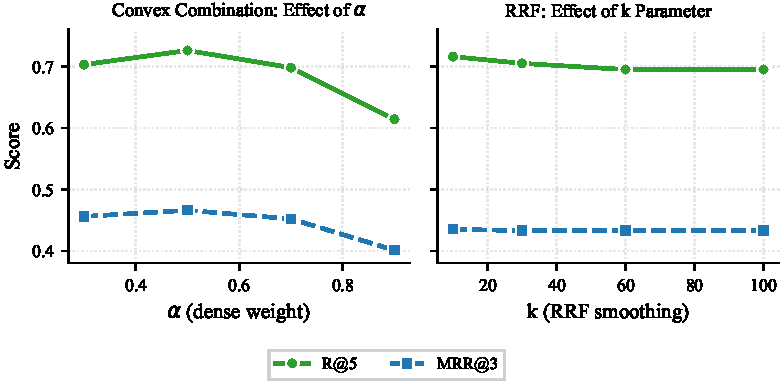
\includegraphics[width=\textwidth]{figures/fusion_ablation.pdf}
\caption{Fusion method ablation. Left: Convex Combination with varying $\alpha$; $\alpha = 0.5$ is optimal. Right: RRF with varying $k$; lower $k$ yields better results.}
\label{fig:fusion_ablation}
\end{figure*}

\begin{figure}[t]
\centering
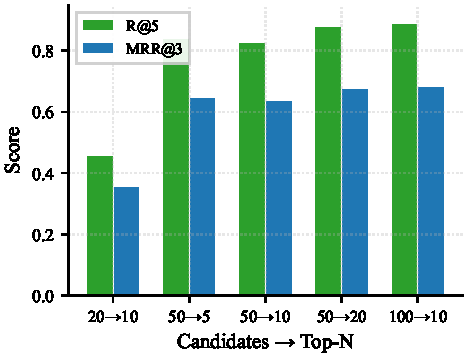
\includegraphics[width=\columnwidth]{figures/reranker_depth.pdf}
\caption{Reranker depth ablation. Critical threshold at 50 candidates.}
\label{fig:reranker_depth}
\end{figure}

% ============================================================
\section{Error Taxonomy for Text-and-Table Retrieval}
\label{sec:errors}

The 31.1\% of queries where hybrid RRF misses the gold document in its top-5 is not a uniform error surface. We sampled 100 of those 7{,}188 failures and had GPT-5.4 label each by failure type; the resulting distribution (Table~\ref{tab:errors}) is dominated by a single category.

\begin{table}[t]
\centering
\small
\begin{tabular}{lr}
\toprule
\textbf{Failure Category} & \textbf{\%} \\
\midrule
Table structure mismatch   & 73 \\
Numerical reasoning        & 20 \\
Vocabulary mismatch        &  5 \\
Ambiguous query            &  1 \\
Long document              &  1 \\
\bottomrule
\end{tabular}
\vspace{4pt}
\caption{Error taxonomy ($n{=}100$ sampled failures). Table structure mismatch dominates.}
\label{tab:errors}
\end{table}

\paragraph{Table structure mismatch (73\%).} Standard encoders see a table as linearized text; the two-dimensional row/column geometry is gone by the time the embedding is computed. A query like ``What was net income in 2019?'' cannot match a row whose label (``net income'') and fiscal year (``2019'') sit in different cells of the same row. This is the open problem the benchmark surfaces: table-aware embeddings or retrievers that preserve row/column structure.

\paragraph{Numerical reasoning (20\%)} failures occur when questions require computation (e.g., year-over-year change) rather than direct lookup.

\paragraph{Cross-subset patterns.} TAT-DQA has the highest failure rate (35.6\% vs.\ 27.2\% FinQA, 26.0\% ConvFinQA). Among failures, 71.0\% of gold documents appear in \emph{neither} the dense nor BM25 top-5---genuinely hard cases, not fusion artifacts.

\paragraph{Implications for evaluation.} A method that pushes aggregate Recall@5 up might only be chipping at the vocabulary-mismatch tail (5\% of errors) while leaving the table-structure mass (73\%) untouched. Future evaluations on heterogeneous corpora should split metrics by failure category; the aggregate alone is misleading.

% ============================================================
\section{Discussion}
\label{sec:discussion}

\paragraph{Why BM25 wins, and what that means for leaderboards.}
\texttt{text-embedding-3-large} is in the top tier on MTEB and BEIR, but on T\textsuperscript{2}-RAGBench BM25 beats it on every metric except Recall@20, where the two are tied. The reason is not mysterious: financial queries are full of terms that appear verbatim in their answer documents---company names, tickers, standardized metric labels, fiscal-period identifiers---and lexical matching picks these up cleanly. A dense encoder smears the same tokens into a neighborhood of near-synonyms, many of which the query never asked for. The lesson is narrower than ``rethink evaluation'': MTEB and BEIR rankings simply do not transfer to text-and-table corpora, so do not pick a dense encoder by leaderboard position if that is where your data lives.

\paragraph{The BM25 advantage is robust to encoder choice---and dense fusion is not.}
Swapping \texttt{text-embedding-3-large} for the open-weight BGE-M3 (1024-d) does not flip the ranking. BGE-M3 dense reaches Recall@5 = 0.508, well below OpenAI dense at 0.587 and below BM25 at 0.644. More striking, \emph{adding BGE-M3 to BM25 via RRF gives no gain over BM25 alone} (R@5 = 0.633 vs.\ 0.644, $-1.1$~pp), whereas the same fusion with OpenAI dense yields $+5.1$~pp over BM25 (0.695 vs.\ 0.644). The closed two-stage pipeline (Hybrid + Cohere Rerank, R@5 = 0.816) is also not closely tracked by its open counterpart (Hybrid (BGE-M3) + BGE Rerank, R@5 = 0.611): even after normalising by candidate-pool ceiling, the open reranker recovers 75\% of its top-20 ceiling versus 93\% for Cohere. We do not claim this gap is intrinsic to open weights; \texttt{bge-reranker-v2-m3} is run at its officially recommended \texttt{max\_length}=512, while Cohere uses 4096 tokens. Operating each at its trained point is the most defensible comparison we can offer without retraining, but it does mean the rerankers see different amounts of context per (query, document) pair. The structural takeaway holds in either reading: lexical matching wins on text-and-table data because the answer-bearing tokens occur verbatim, and the marginal value of dense fusion depends on the encoder, not just on whether dense signals are present at all.

\paragraph{The reranker does most of the heavy lifting.}
Adding a cross-encoder reranker on top of hybrid RRF is worth +17.2pp MRR@3 and +12.1pp Recall@5. That is a larger improvement than anything else we measured, and it is the only configuration that closes most of the gap to the oracle ceiling. Candidate depth matters: the rerank step degrades below 50 candidates (Section~\ref{sec:ablations}).

\paragraph{If you have to pick one setup.}
Use hybrid RRF with a cross-encoder reranker and a candidate pool of at least 50. Contextual retrieval is worth the one-time indexing cost: it lifts both dense and hybrid by roughly 2--3 pp of Recall@5 for an LLM call per document. Skip HyDE and multi-query for numerical domains---HyDE actively moves the numbers in the wrong direction, and multi-query does not close the gap to BM25. And do not extrapolate from MTEB/BEIR; evaluate on data that looks like yours.

% ============================================================
\section{Conclusion}
\label{sec:conclusion}

On a financial QA benchmark of 23{,}088 text-and-table queries, hybrid RRF followed by a cross-encoder reranker delivers the best end-to-end performance; stacking query expansion on top of a dense encoder makes things worse. Two findings are worth carrying to other heterogeneous corpora. BM25 beats a state-of-the-art dense encoder on nearly every metric, so MTEB and BEIR rankings should not be taken as guidance for data this isn't drawn from. And 73\% of the retrieval failures that remain share a single cause: the answer is a table cell, and the encoder processes tables as serialized text. Closing that gap is less about scaling the encoder than about representing tabular structure---natural candidates are late-interaction retrievers (ColBERTv2~\citep{santhanam2022colbertv2}, Jina-ColBERT-v2~\citep{sturua2024jinacolbert}) and structure-aware chunking strategies that we did not explore here.

% ============================================================
\section*{Limitations}

\paragraph{One domain.} The corpus is financial filings. A different domain mix---legal briefs with tables, medical records, scientific papers---may shift both the absolute numbers and the ordering between methods, though we expect BM25's edge to be strongest where terminology is standardized and weakest where paraphrase is common.

\paragraph{Numerical-only answers.} Every answer in T\textsuperscript{2}-RAGBench is a number, which is why Number Match is the primary generation metric. We do not test whether the same retrieval ordering holds for free-form answers.

\paragraph{Whole-document retrieval.} We index each document whole ($\sim$920 tokens). Chunking changes the recall game; it may close part of the dense-encoder gap on longer documents by giving the encoder a smaller surface to summarize.

\paragraph{Two dense encoders, two rerankers.} We evaluated two dense encoders (\texttt{text-embedding-3-large}, BGE-M3) and two cross-encoder rerankers (Cohere Rerank v4.0 Pro, \texttt{bge-reranker-v2-m3}). The qualitative ordering---BM25 above either dense encoder, hybrid above both, hybrid+rerank above hybrid for the closed stack---held in every pairing we tested. Encoder families with explicit table-structure pretraining (e.g.\ table-aware contrastive variants) may behave differently. The two rerankers are run at different officially recommended \texttt{max\_length} settings (4{,}096 vs.\ 512); we do not claim universality across reranker context windows.

\paragraph{Commercial APIs.} The dense encoder, reranker, and generation LLM are all commercial endpoints. Model weights and behaviors can change. We release per-query outputs so that our results can be compared against future re-runs rather than re-reproduced from scratch.

% ============================================================
\section*{Ethics Statement}

The source data is public---SEC filings, accessed through the T\textsuperscript{2}-RAGBench release. No personal, private, or human-subject data is used, and all LLM calls go through commercial endpoints under their standard terms. The main positive externality we expect is cheaper, more accurate retrieval in RAG systems built over regulatory or financial documents; the main negative externality to flag is that better retrieval over SEC filings could make it easier to automate certain information-asymmetry exploits (e.g., faster-than-human extraction of earnings figures for algorithmic trading). The mitigation is identical to the existing state of the art---these documents are already public, and practitioners can already search them. Releasing a stronger retrieval baseline does not change who has access; it changes only how fast the useful signal can be surfaced.

% ============================================================
% Acknowledgments omitted for double-blind review; will be added in the camera-ready version.

\bibliographystyle{plainnat}
\bibliography{references}

\section*{NeurIPS Paper Checklist}

\begin{enumerate}

\item {\bf Claims}
    \item[] Question: Do the main claims made in the abstract and introduction accurately reflect the paper's contributions and scope?
    \item[] Answer: \answerYes{}
    \item[] Justification: The abstract and introduction (Section~\ref{sec:intro}) state five specific contributions, all of which are supported by experimental results in Sections~\ref{sec:results}--\ref{sec:negative}. Limitations are discussed explicitly.

\item {\bf Limitations}
    \item[] Question: Does the paper discuss the limitations of the work performed by the authors?
    \item[] Answer: \answerYes{}
    \item[] Justification: A dedicated Limitations section covers domain specificity (financial only), answer-type bias (numerical only), document granularity (whole-document retrieval), embedding-model coverage (one dense encoder), and API dependency.

\item {\bf Theory assumptions and proofs}
    \item[] Question: For each theoretical result, does the paper provide the full set of assumptions and a complete (and correct) proof?
    \item[] Answer: \answerNA{}
    \item[] Justification: This is an empirical benchmarking paper with no theoretical results or proofs.

    \item {\bf Experimental result reproducibility}
    \item[] Question: Does the paper fully disclose all the information needed to reproduce the main experimental results of the paper to the extent that it affects the main claims and/or conclusions of the paper (regardless of whether the code and data are provided or not)?
    \item[] Answer: \answerYes{}
    \item[] Justification: Section~\ref{sec:setup} describes the experimental setup. Appendix~\ref{app:hyperparams} provides complete hyperparameter tables. Appendix~\ref{app:prompts} provides all prompt templates. The dataset is publicly available. Random seed, temperature, and all configuration details are specified.


\item {\bf Open access to data and code}
    \item[] Question: Does the paper provide open access to the data and code, with sufficient instructions to faithfully reproduce the main experimental results, as described in supplemental material?
    \item[] Answer: \answerYes{}
    \item[] Justification: The benchmark code and evaluation scripts are released as an open-source repository. The dataset (T\textsuperscript{2}-RAGBench) is publicly available from the original authors.

\item {\bf Experimental setting/details}
    \item[] Question: Does the paper specify all the training and test details (e.g., data splits, hyperparameters, how they were chosen, type of optimizer) necessary to understand the results?
    \item[] Answer: \answerYes{}
    \item[] Justification: Section~\ref{sec:setup} describes infrastructure, document representation, and reproducibility measures. Appendix~\ref{app:hyperparams} provides a complete hyperparameter table for all methods. We use the standard train/test split from the original benchmark.

\item {\bf Experiment statistical significance}
    \item[] Question: Does the paper report error bars suitably and correctly defined or other appropriate information about the statistical significance of the experiments?
    \item[] Answer: \answerYes{}
    \item[] Justification: All pairwise method comparisons use paired bootstrap tests ($B = 10{,}000$) with Bonferroni correction at $p < 0.05$ (Section~\ref{sec:metrics}). Significance levels are reported alongside all main results.

\item {\bf Experiments compute resources}
    \item[] Question: For each experiment, does the paper provide sufficient information on the computer resources (type of compute workers, memory, time of execution) needed to reproduce the experiments?
    \item[] Answer: \answerYes{}
    \item[] Justification: Section~\ref{sec:setup} describes the compute setup: BM25 and FAISS run locally on Apple Silicon; embedding, LLM, and reranking calls use Azure AI Foundry. No GPU training is required to reproduce the main results.

\item {\bf Code of ethics}
    \item[] Question: Does the research conducted in the paper conform, in every respect, with the NeurIPS Code of Ethics \url{https://neurips.cc/public/EthicsGuidelines}?
    \item[] Answer: \answerYes{}
    \item[] Justification: The research uses publicly available data (SEC filings), does not involve human subjects, and poses no foreseeable ethical concerns. An Ethics Statement is included.

\item {\bf Broader impacts}
    \item[] Question: Does the paper discuss both potential positive societal impacts and negative societal impacts of the work performed?
    \item[] Answer: \answerYes{}
    \item[] Justification: The Ethics Statement discusses both sides: the positive externality of cheaper, more accurate retrieval in RAG systems over regulatory and financial documents, and the negative externality that stronger retrieval on SEC filings could accelerate information-asymmetry exploits (e.g., algorithmic earnings extraction). It notes that the data is already public, so the release does not change access, only speed.

\item {\bf Safeguards}
    \item[] Question: Does the paper describe safeguards that have been put in place for responsible release of data or models that have a high risk for misuse (e.g., pre-trained language models, image generators, or scraped datasets)?
    \item[] Answer: \answerNA{}
    \item[] Justification: This paper does not release new models or datasets. The released code is an evaluation framework with no misuse risk.

\item {\bf Licenses for existing assets}
    \item[] Question: Are the creators or original owners of assets (e.g., code, data, models), used in the paper, properly credited and are the license and terms of use explicitly mentioned and properly respected?
    \item[] Answer: \answerYes{}
    \item[] Justification: All datasets (FinQA, ConvFinQA, TAT-DQA, T\textsuperscript{2}-RAGBench) and models are cited with their original papers. The benchmark is used under its original license terms.

\item {\bf New assets}
    \item[] Question: Are new assets introduced in the paper well documented and is the documentation provided alongside the assets?
    \item[] Answer: \answerYes{}
    \item[] Justification: The evaluation framework code is released with documentation, configuration files, and instructions for reproducing all experiments.

\item {\bf Crowdsourcing and research with human subjects}
    \item[] Question: For crowdsourcing experiments and research with human subjects, does the paper include the full text of instructions given to participants and screenshots, if applicable, as well as details about compensation (if any)?
    \item[] Answer: \answerNA{}
    \item[] Justification: This paper does not involve crowdsourcing or research with human subjects.

\item {\bf Institutional review board (IRB) approvals or equivalent for research with human subjects}
    \item[] Question: Does the paper describe potential risks incurred by study participants, whether such risks were disclosed to the subjects, and whether Institutional Review Board (IRB) approvals (or an equivalent approval/review based on the requirements of your country or institution) were obtained?
    \item[] Answer: \answerNA{}
    \item[] Justification: This paper does not involve human subjects research.

\item {\bf Declaration of LLM usage}
    \item[] Question: Does the paper describe the usage of LLMs if it is an important, original, or non-standard component of the core methods in this research? Note that if the LLM is used only for writing, editing, or formatting purposes and does \emph{not} impact the core methodology, scientific rigor, or originality of the research, declaration is not required.
    \item[] Answer: \answerYes{}
    \item[] Justification: LLMs are core components of several retrieval methods (HyDE, Multi-Query, CRAG, Contextual Retrieval) and the generation evaluation stage. All LLM usage is documented in Sections~\ref{sec:methods}--\ref{sec:generation} with model names, temperatures, and exact prompts in Appendix~\ref{app:prompts}.

\end{enumerate}


\appendix

\section{Hyperparameter Details and Full Results}
\label{app:hyperparams}

Table~\ref{tab:hyperparams} lists all hyperparameters. Table~\ref{tab:full_results} presents full retrieval metrics. Table~\ref{tab:subset_results} shows per-subset performance.

\begin{table*}[!t]
\centering
\scriptsize
\setlength{\tabcolsep}{4pt}
\begin{tabular}{@{}llll@{}}
\toprule
\textbf{Method} & \textbf{Parameter} & \textbf{Value} & \textbf{Notes} \\
\midrule
\multirow{2}{*}{BM25}
  & $k_1$ / $b$      & 1.2 / 0.75 & Canonical Okapi defaults \\
  & Tokenizer        & whitespace split & Via \texttt{rank\_bm25} \\
\midrule
\multirow{3}{*}{Dense (text-embed-3-large)}
  & Dimensions       & 3{,}072 & OpenAI via Azure AI Foundry \\
  & Max input        & $\sim$8{,}191 tokens & API default \\
  & Index type       & FAISS \texttt{IndexFlatIP} & Exact cosine search \\
\midrule
\multirow{3}{*}{Dense (BGE-M3)\textsuperscript{$\diamond$}}
  & Dimensions       & 1{,}024 & \texttt{BAAI/bge-m3} via \texttt{sentence-transformers} \\
  & \texttt{max\_seq\_length} & 8{,}192 & BGE-M3 native maximum \\
  & Index type       & FAISS \texttt{IndexFlatIP} & Exact cosine search \\
\midrule
Hybrid RRF & $k$ & 60 (ablation: 10, 30, 100) & Smoothing constant \\
\midrule
Hybrid CC & $\alpha$ & 0.5 (ablation: 0.3, 0.7, 0.9) & Dense weight \\
\midrule
\multirow{3}{*}{Cohere Rerank}
  & Model / top\_n   & v4.0-pro / 10 & Via Azure AI Foundry \\
  & \texttt{max\_tokens\_per\_doc} & 4{,}096 & API default \\
  & Candidate pool   & 50    & From first stage \\
\midrule
\multirow{3}{*}{BGE Rerank\textsuperscript{$\diamond$}}
  & Model / top\_n   & \texttt{bge-reranker-v2-m3} / 10 & Local cross-encoder \\
  & \texttt{max\_length} & 512 & Official recommended default \\
  & Candidate pool   & 60 & From first stage; minor asymmetry vs Cohere (50) \\
\midrule
HyDE & LLM / temp / max\_tok & gpt-4.1-mini / 0 / 150 & Single generation \\
\midrule
Multi-Query & Variants / RRF $k$ & 3 / 60 & gpt-4.1-mini, temp 0 \\
\midrule
CRAG & Eval temp / rewrite temp & 0.0 / 0.5 & gpt-4.1-mini \\
\midrule
Contextual & LLM / temp / max\_tok & gpt-4.1-mini / 0 / 100 & Per-document context \\
\midrule
\multirow{2}{*}{Global}
  & Seed / top-$k$ & 42 / \{1,3,5,10,20\} & All methods \\
  & Bootstrap & $B{=}10{,}000$, $p{<}0.05$ & Bonferroni-corrected \\
\bottomrule
\end{tabular}
\vspace{4pt}
\caption{Complete hyperparameter settings for all retrieval methods.}
\label{tab:hyperparams}
\end{table*}

\begin{table*}[!t]
\centering
\small
\setlength{\tabcolsep}{4.5pt}
\begin{tabular}{lcccccccccc}
\toprule
\textbf{Method} & \textbf{R@1} & \textbf{R@3} & \textbf{R@5} & \textbf{R@10} & \textbf{R@20} & \textbf{MRR@3} & \textbf{MRR@5} & \textbf{nDCG@5} & \textbf{nDCG@10} & \textbf{MAP} \\
\midrule
Dense (BGE-M3)\textsuperscript{$\diamond$}
                  & 0.225 & 0.425 & 0.508 & 0.597 & 0.677 & 0.315 & 0.334 & 0.377 & 0.406 & 0.351 \\
HyDE              & 0.221 & 0.441 & 0.544 & 0.671 & 0.767 & 0.318 & 0.341 & 0.392 & 0.433 & 0.365 \\
Dense             & 0.248 & 0.481 & 0.587 & 0.703 & 0.798 & 0.351 & 0.375 & 0.428 & 0.466 & 0.398 \\
Contextual Dense  & 0.266 & 0.508 & 0.615 & 0.732 & 0.817 & 0.373 & 0.398 & 0.452 & 0.490 & 0.420 \\
Hybrid (BGE-M3) + BGE Rerank\textsuperscript{$\diamond$}
                  & 0.301 & 0.537 & 0.611 & 0.693 & 0.764 & 0.409 & 0.426 & 0.472 & 0.499 & 0.442 \\
Hybrid (BGE-M3)\textsuperscript{$\diamond$}
                  & 0.286 & 0.538 & 0.633 & 0.733 & 0.814 & 0.399 & 0.421 & 0.474 & 0.507 & 0.440 \\
Multi-Query       & 0.283 & 0.539 & 0.640 & 0.734 & 0.820 & 0.397 & 0.420 & 0.475 & 0.506 & 0.439 \\
BM25              & 0.293 & 0.552 & 0.644 & 0.735 & 0.797 & 0.411 & 0.432 & 0.485 & 0.515 & 0.449 \\
CRAG              & 0.302 & 0.556 & 0.658 & 0.788 & 0.788\textsuperscript{$\dagger$} & 0.415 & 0.439 & 0.493 & 0.536 & 0.456 \\
Hybrid RRF        & 0.308 & 0.588 & 0.695 & 0.801 & 0.877 & 0.433 & 0.457 & 0.517 & 0.551 & 0.477 \\
Contextual Hybrid & 0.327 & 0.610 & 0.717 & 0.818 & 0.887 & 0.454 & 0.478 & 0.538 & 0.571 & 0.497 \\
Hybrid + Rerank   & \textbf{0.472} & \textbf{0.758} & \textbf{0.816} & \textbf{0.861} & \textsuperscript{$\ast$} & \textbf{0.605} & \textbf{0.618} & \textbf{0.669} & \textbf{0.683} & \textbf{0.625} \\
\bottomrule
\end{tabular}
\vspace{4pt}
\caption{Full retrieval results, sorted by nDCG@10. Rows marked \textsuperscript{$\diamond$}~use the open-weight \texttt{BAAI/bge-m3}~+~\texttt{bge-reranker-v2-m3} stack; all other rows use \texttt{text-embedding-3-large}. \textsuperscript{$\ast$}Rerank returns $\leq$10 docs. \textsuperscript{$\dagger$}CRAG returns $\leq$10 documents; R@20 reported equal to R@10 for completeness.}
\label{tab:full_results}
\end{table*}

\begin{table}[!t]
\centering
\small
\begin{tabular}{llccc}
\toprule
\textbf{Subset} & \textbf{Method} & \textbf{R@5} & \textbf{R@10} & \textbf{MRR@3} \\
\midrule
\multirow{5}{*}{FinQA}
  & BM25    & 0.729 & 0.834 & 0.389 \\
  & Dense   & 0.611 & 0.748 & 0.308 \\
  & Hybrid  & \textbf{0.737} & \textbf{0.856} & \textbf{0.389} \\
  & Dense (BGE-M3)\textsuperscript{$\diamond$}    & 0.600 & 0.703 & 0.365 \\
  & Hybrid (BGE-M3) + BGE Rerank\textsuperscript{$\diamond$} & 0.660 & 0.754 & 0.393 \\
\midrule
\multirow{5}{*}{ConvFinQA}
  & BM25    & 0.696 & 0.781 & 0.500 \\
  & Dense   & 0.654 & 0.781 & 0.410 \\
  & Hybrid  & \textbf{0.754} & \textbf{0.850} & \textbf{0.519} \\
  & Dense (BGE-M3)\textsuperscript{$\diamond$}    & 0.582 & 0.677 & 0.330 \\
  & Hybrid (BGE-M3) + BGE Rerank\textsuperscript{$\diamond$} & 0.687 & 0.759 & 0.492 \\
\midrule
\multirow{5}{*}{TAT-DQA}
  & BM25    & 0.566 & 0.649 & 0.400 \\
  & Dense   & 0.549 & 0.647 & 0.364 \\
  & Hybrid  & \textbf{0.647} & \textbf{0.746} & \textbf{0.438} \\
  & Dense (BGE-M3)\textsuperscript{$\diamond$}    & 0.418 & 0.496 & 0.274 \\
  & Hybrid (BGE-M3) + BGE Rerank\textsuperscript{$\diamond$} & 0.551 & 0.628 & 0.395 \\
\bottomrule
\end{tabular}
\vspace{4pt}
\caption{Per-subset results. TAT-DQA is hardest; hybrid RRF gains most on TAT-DQA (+8.1pp R@5 over BM25). Rows marked \textsuperscript{$\diamond$}~use the open-weight \texttt{BAAI/bge-m3}~+~\texttt{bge-reranker-v2-m3} stack.}
\label{tab:subset_results}
\end{table}

\section{Additional Figures}
\label{app:figures}

\begin{figure*}[!t]
\centering
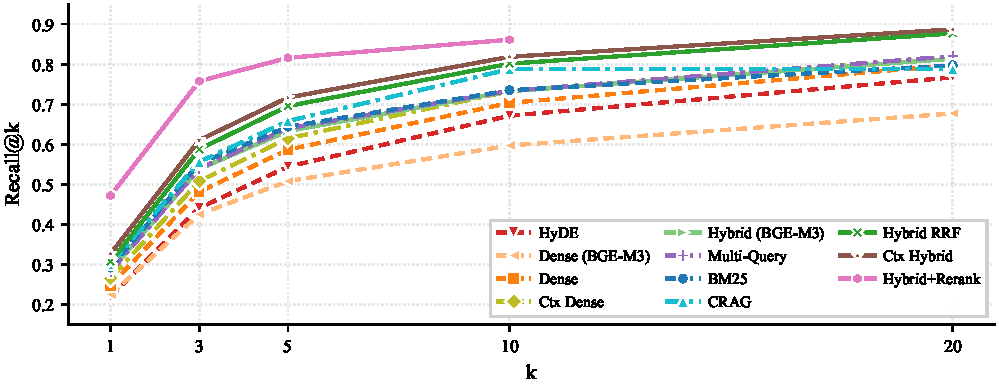
\includegraphics[width=\textwidth]{figures/recall_at_k.pdf}
\caption{Recall@$k$ curves. Hybrid fusion outperforms both baselines at every $k$, with the largest gains at small $k$.}
\label{fig:recall_curve}
\end{figure*}

\begin{figure*}[!t]
\centering
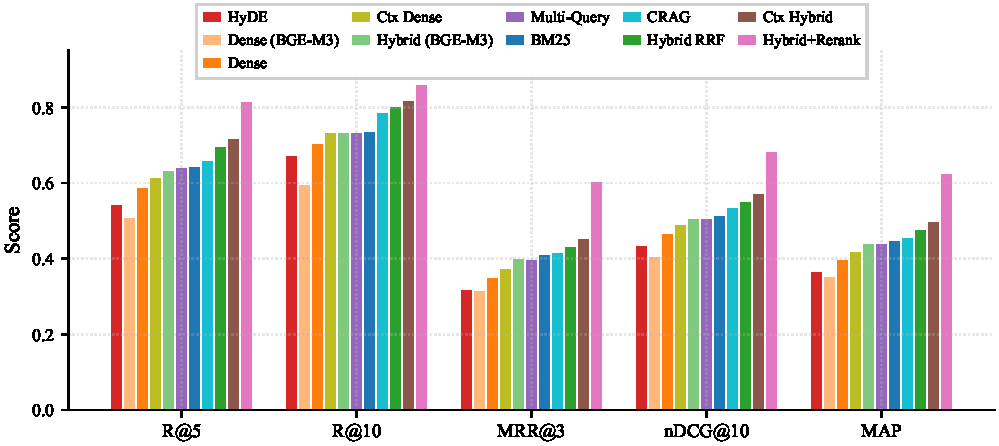
\includegraphics[width=\textwidth]{figures/main_comparison.pdf}
\caption{Grouped comparison across five metrics. BM25 outperforms dense retrieval; hybrid RRF dominates.}
\label{fig:bar_comparison}
\end{figure*}

\begin{figure}[!t]
\centering
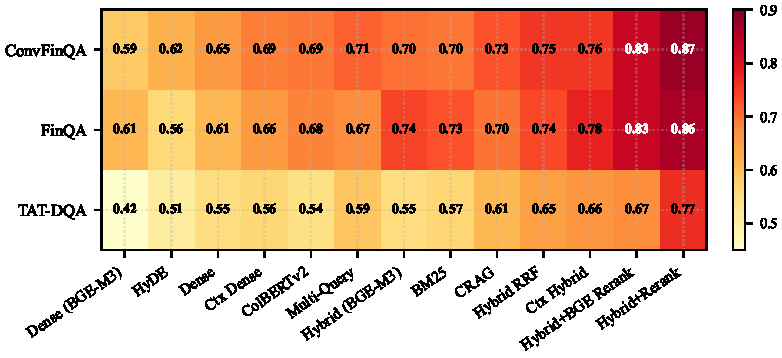
\includegraphics[width=\columnwidth]{figures/subset_heatmap.pdf}
\caption{Recall@5 heatmap across methods and subsets. TAT-DQA is consistently hardest.}
\label{fig:heatmap}
\end{figure}

\begin{figure}[!t]
\centering
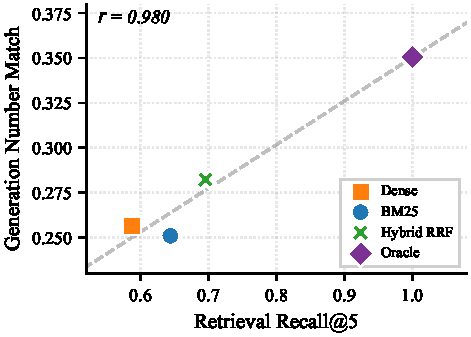
\includegraphics[width=\columnwidth]{figures/retrieval_generation_correlation.pdf}
\caption{Retrieval--generation correlation ($r > 0.99$): better retrieval leads to better answers.}
\label{fig:correlation}
\end{figure}

% ============================================================
\section{Prompt Templates}
\label{app:prompts}

All prompts use \texttt{gpt-4.1-mini} via Azure AI Foundry.

\subsection{Generation Prompt}
\begin{small}
\begin{verbatim}
Answer the following question based ONLY on
the provided context.
If the answer is a number, provide just the
number. If you cannot answer from the
context, say "UNANSWERABLE".

Context: {context}
Question: {question}
Answer:
\end{verbatim}
\end{small}

\subsection{HyDE Prompt}
\begin{small}
\begin{verbatim}
Given the following question about financial
data, write a short passage that would
contain the answer. Include specific numbers
and financial terms.
Question: {query}
Passage:
\end{verbatim}
\end{small}

\subsection{Multi-Query Prompt}
\begin{small}
\begin{verbatim}
You are a helpful assistant that generates
alternative search queries. Given the
following question, generate {n} alternative
phrasings that capture the same information
need but use different wording or
perspectives. Return each query on its own
line, numbered. Do not include any other text.

Original question: {query}
Alternative queries:
\end{verbatim}
\end{small}

\subsection{CRAG Evaluation Prompt}
\begin{small}
\begin{verbatim}
You are a relevance evaluator. Given a
question and a retrieved document, classify
the document's relevance.

Question: {query}
Document: {document}

Respond with exactly one of:
- RELEVANT
- AMBIGUOUS
- IRRELEVANT

Classification:
\end{verbatim}
\end{small}

\subsection{CRAG Rewrite Prompt}
\begin{small}
\begin{verbatim}
The following question was used to search a
financial document corpus, but the retrieved
results were not sufficiently relevant.

Original question: {query}

Please rewrite this question to be more
specific and likely to retrieve the correct
financial document.

Rewritten question:
\end{verbatim}
\end{small}

\subsection{Contextual Retrieval Prompt}
\begin{small}
\begin{verbatim}
Here is a document:
<document>
{document}
</document>

Please provide a concise summary context
(2-3 sentences) that captures the key
topics and entities in this document, for
the purpose of improving search retrieval.
Answer only with the context, nothing else.
\end{verbatim}
\end{small}

\end{document}
